\subsection{Semantic Adaptations}\label{sec:adaptation}

While the FMI standard defines a common format for exchanging FMUs it does not guarantee the absence of so called \emph{interaction mismatches} when these are composed \cite{Gomes&18a}.
The goal of semantic adaptations~(SA), is to allow these mismatches to be corrected without the need to involve the original author of the FMU.

A concrete example where this would be if \emph{valve} input of the \emph{WaterTank} accepted a bool instead of a real.
In this case it would not be possible to connect the \emph{valvecontrol} and \emph{valve} ports.
A SA could be used to apply a threshold to the \emph{valve} output in order to convert it into a bool, as seen in figure~\ref{fig:watertank_SA}.

\begin{figure}[bt]
\centering
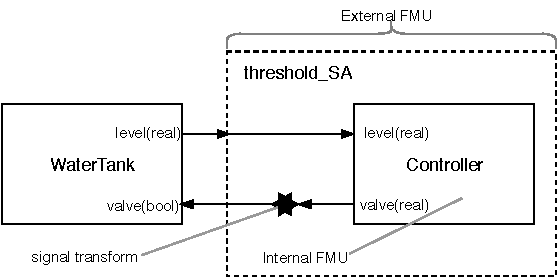
\includegraphics[width=0.8\columnwidth]{Images/watertank_SA.pdf}
\caption{Example of how semantic adaptation may be applied to correct signal data mismatch.}
\label{fig:watertank_SA}
\end{figure}


Conceptually, a SA can be thought of as an \emph{external} FMU, which wraps around one or more \emph{internal} FMUs. The external FMU is responsible for managing the execution of the internal FMUs. In the previous example the external FMU would simply pass all signals directly, except for the \emph{valve}, which would be thresholded before being written to the \emph{valve} output of the external FMU.  
The approach grants a great deal of flexibility, allowing a large number of adaptations to be implemented. In addition, it allows these to be applied in a hierarchical manner, e.g. "on top of" each other.

As described in Section~\ref{sec:intro} the SysML CPS profile does not yet support semantic adaptations \cite{Gomes&18a}. In general such semantics adaptations are currently established by a separate Domain Specific Language (DSL). This is introduced in order to perform different kinds of adaptations to existing FMUs that enable their behaviour to be adjusted in different ways. However, the DSL from \cite{Gomes&18a} also enables support for hierarchical co-simulations. A different approach for hierarchical co-simulations has been introduced in \cite{Thule&19}. 


%This work seeks to find a graphical representation that is easy to apply while remaining sufficiently %expressive.


%Graphically most of these can be represented as different kinds of annotations.

%There are several important differences in concepts and notation used within INTO-CPS toolchain and the SSP.
%A superficial understanding these are essential to following the discussion and design choices of the editor.
%While being designed as a complementary standard for FMI; SSP is agnostic towards the implementation details of a simulation unit.
%To emphasize this its uses the word \emph{component} instead of FMU.
%A crucial detail is that a component may itself be a SSP package \cite[p.53]{SSP19}.
%If this is the case it is referred to as a \emph{subsystem}.
%Another difference is that one SSP package may be contain several so called \emph{systems}.
%In the context of the editor, a system is equivalent to a multi model.
